\documentclass[../../main.tex]{subfiles}

\begin{document}
\problem{31}
\begin{wts}
What is the URI of the requested file?
\end{wts}
\begin{proof}
Consider the following graphic,\\
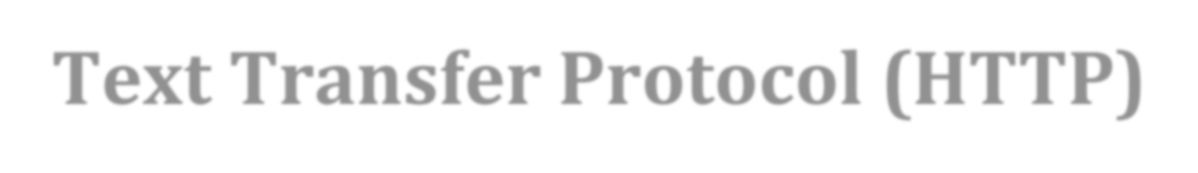
\includegraphics[width=\textwidth]{subfiles/images/L5_Manual/L5N2_ DNS & HTTP_PAGE20_11_Image131.png}
The figure does not contain enough information to make a definitive conclusion. First, we do not know the units for time, whether they are in RTT, ERTT, SRTT, etc. Second, during the periods where the y-axis falls drastically to 1 dimensionless units, we do not know if it is caused by a true timeout or k-duplicate ACKs. Third, the units for the y-axis are missing. Does the MSS change with time during this protocol? This we can never know. To this, we will make three assumptions, one of which will have two cases. And in each of those two cases will yield — unsurprisingly, two different answers.
\begin{itemize}
    \item The axes are unitised with MSS and RTT respectively,
    \item The figure describes a protocol past its Connection Establishment phase,
    \item Either all of the y-drops are caused by timeouts, or none of them are. (And therefore caused by duplicate ACKs).
\end{itemize}

It is only after unveiling the ambiguity in the question, that anyone with his or her eyes open would be able to tell that the figure employs TCP Reno or Tahoe (exclusively at once), and TCP Tahoe. The discussion that follows assumes that all units of time are given in the discrete multiples of RTT, whereby assuming a symmetric LTI channel, and cwnd in multiples of MSS.\\

In a word, the operation of TCP Reno is based on the ability for the transmitter to distinguish between packets which are lost due to a timeout, which occurs only if multiple packets were lost during RTT — and packets which are lost individually. In the first case, TCP Reno sets ${ss}_{thresh}$ = cwnd/2, and — by invoking our second assumption —, resets cwnd to 1. On the subsequent RTT, TCP Reno is configured to be in Slow Start (terminating after cwnd=${ss}_{thresh}$) upon the immediate retransmission of the oldest lost segment.\\

In the second case, TCP Reno sets ${ss}_{thresh}$ = cwnd/2, and slashes cwnd by half. After retransmitting the lost segment, TCP Reno resumes using AIMD.\\

TCP Tahoe, does not distinguish between the two cases, and employs the second method of control, without regard whether the packets were lost in the atomic sense, or in unison.\\

Finally, both protocols are configured to start in Slow Start, with ${ss}_{thresh}$ ‘at infinity’ (in mathematical terms, taking ${ss}_{thresh}$ to be least of the ordinals that are greater — as directed by inclusion — than every initial segment of the first countable ordinals would suffice), and cwnd = 1.
\end{proof}

\end{document}